\begin{frame}[c]{}

\centering
\huge
Lecture 8+9:\\
Meta-Learning I+II
\end{frame}
%----------------------------------------------------------------------
\begin{frame}[c]{Where are we? The big picture}

\begin{itemize}
	\item Introduction
	\item Background
	\begin{itemize}
		\item Design spaces in ML
		\item Evaluation and visualization
	\end{itemize}
	\item[$\to$] Hyperparameter optimization (HPO)
	\begin{itemize}
		\item Bayesian optimization
		\item Other black-box techniques
		\item Speeding up HPO with multi-fidelity optimization
	\end{itemize}
	\item Pentecost (Holiday) -- no lecture
	\item Architecture search I + II
	\item[$\to$] Meta-Learning I ++ II
	\item Beyond AutoML: algorithm configuration and control
	\item Project announcement and closing
\end{itemize}

\end{frame}
%----------------------------------------------------------------------

%----------------------------------------------------------------------
\begin{frame}[c]{Learning Goals}

After this lecture, you will be able to \ldots

\begin{itemize}
	\item ...
\end{itemize}

\end{frame}
%-----------------------------------------------------------------------
%----------------------------------------------------------------------
\begin{frame}[c]{Further Material}

There were two great tutorials on meta-learning recently:

\begin{itemize}
	\item NeurIPS'18: Frank Hutter and Joaquin Vanschoren
	"Automatic Machine Learning (AutoML): A Tutorial"
	\url{https://videoken.com/embed/5A4xbv5nd8c}
	\item ICML'19: Chelsea Finn and Sergey Levine on\\
	"Meta-Learning: from Few-Short Learning to Rapid Reinforcement Learning"\\
	\url{https://www.facebook.com/icml.imls/videos/400619163874853/}
\end{itemize}

\begin{itemize}
	\item Strong recommendation to watch both tutorials
	\item We can't cover all the stuff today
	\item Parts of the material used today was inspired by these tutorials
\end{itemize}


\end{frame}
%-----------------------------------------------------------------------
\section{Meta-Learning}
%----------------------------------------------------------------------
\begin{frame}[c]{The Idea of Meta-Learning}

\begin{itemize}
	\item Learning essential never stops
	\begin{itemize}
		\item We learn several models on the same task (e.g., dataset)
		\item We learn models on new tasks
	\end{itemize}
    \pause
    \item Learning is often done from scratch
    \item[$\leadsto$] We humans don't start from scratch all the time,
    but we learned how to learn!
\end{itemize}

\bigskip

\begin{tikzpicture}

	\node (task1) [data, text width=6em] {Task~1};
	\node (learn1) [activity, below of=task1, text width=6em] {Learning};
	\node (models1) [activity, below of=learn1, text width=6em] {Models};
	\node (perf1) [data, below of=models1, text width=6em] {Performance};
	
	\node (task2) [data, right of=task1, node distance=4.5cm, text width=6em] {Task~2};
	\node (learn2) [activity, below of=task2, text width=6em] {Learning};
	\node (models2) [activity, below of=learn2, text width=6em] {Models};
	\node (perf2) [data, below of=models2, text width=6em] {Performance};
	
	\node (task3) [data, right of=task2, node distance=4.5cm, text width=6em] {Task~3};
	\node (learn3) [activity, below of=task3, text width=6em] {Learning};
	\node (models3) [activity, below of=learn3, text width=6em] {Models};
	\node (perf3) [data, below of=models3, text width=6em] {Performance};
	
	\draw[myarrow] (task1) -- (learn1);
	\draw[myarrow] (learn1) -- (task1);
	\draw[myarrow] (learn1) -- (models1);
	\draw[myarrow] (models1) -- (perf1);
	
	\draw[myarrow] (task2) -- (learn2);
	\draw[myarrow] (learn2) -- (task2);
	\draw[myarrow] (learn2) -- (models2);
	\draw[myarrow] (models2) -- (perf2);
	
	\draw[myarrow] (task3) -- (learn3);
	\draw[myarrow] (learn3) -- (task3);
	\draw[myarrow] (learn3) -- (models3);
	\draw[myarrow] (models3) -- (perf3);
	
	\draw[myarrow] (learn1) -- node[above] {Meta-Learn} (learn2);
	\draw[myarrow] (learn2) -- node[above] {Meta-Learn} (learn3);	
\end{tikzpicture}

\end{frame}
%-----------------------------------------------------------------------
\begin{frame}[c]{Example for Human Meta-Learning}

\begin{columns}
	\column{0.18\textwidth}
	Braque
	\centering
	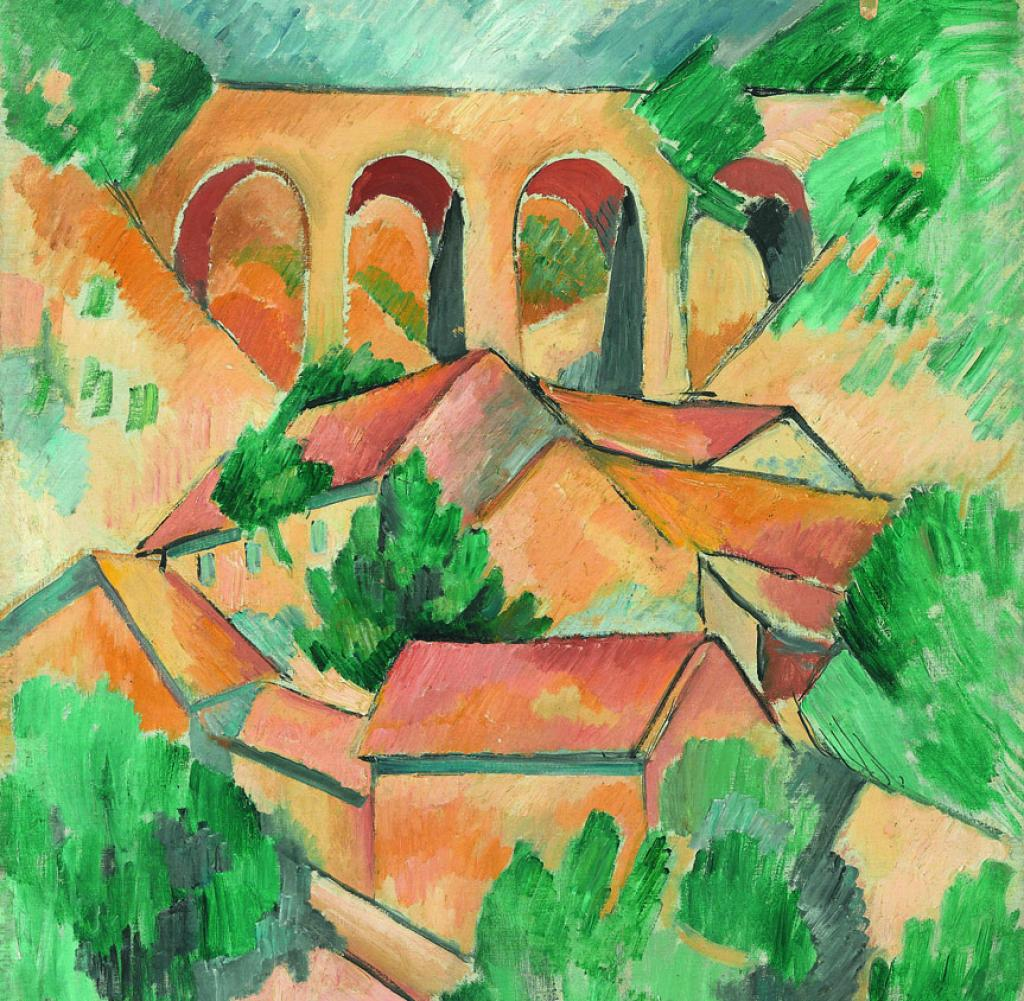
\includegraphics[width=1.0\textwidth]{images/braque1.jpg}
	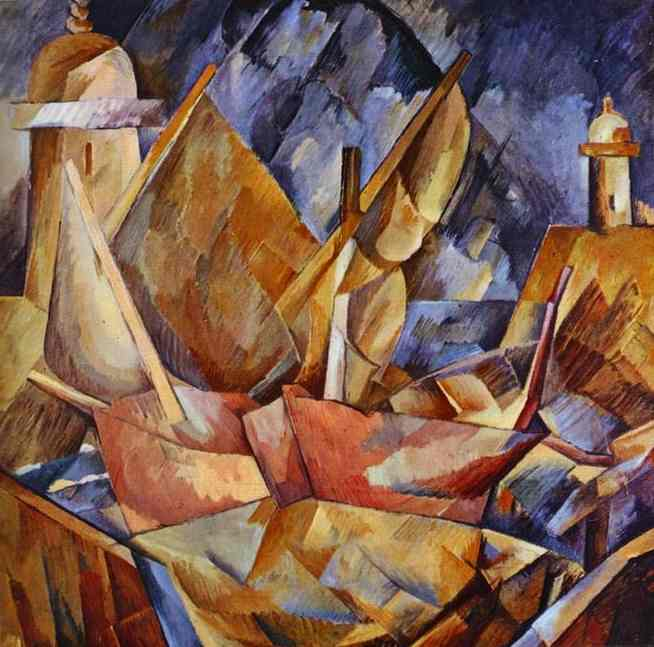
\includegraphics[width=1.0\textwidth]{images/braque2.jpeg}
	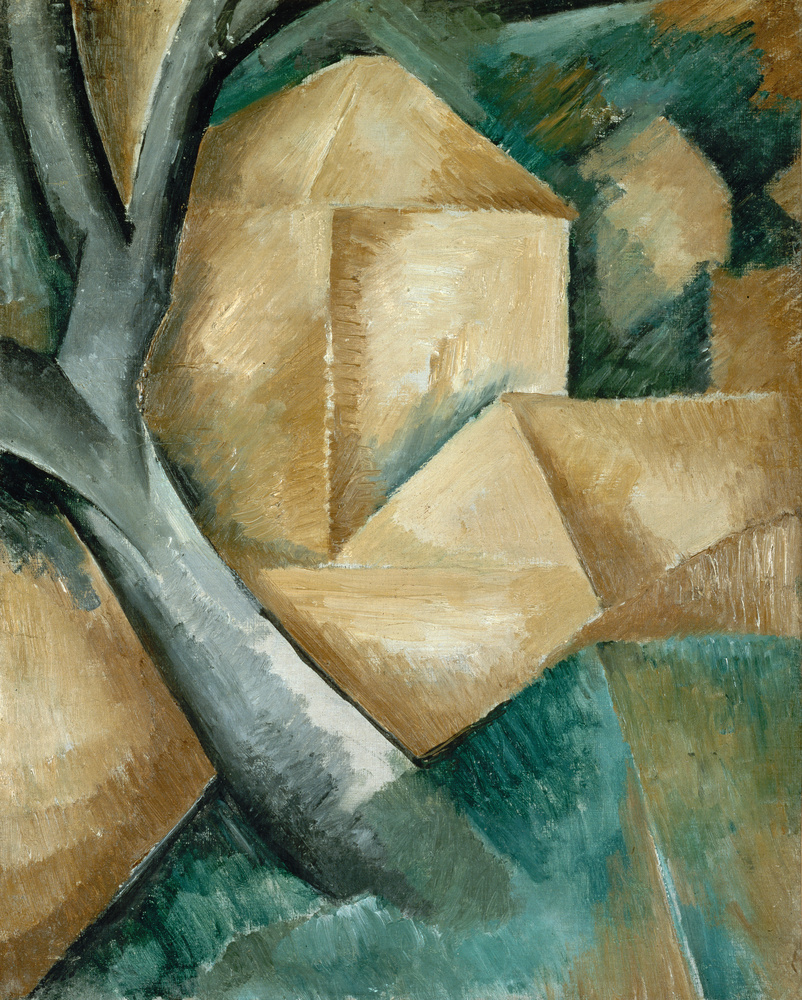
\includegraphics[width=1.0\textwidth]{images/braque3.jpg}
	\column{0.258\textwidth}
	Cezanne
	\centering
	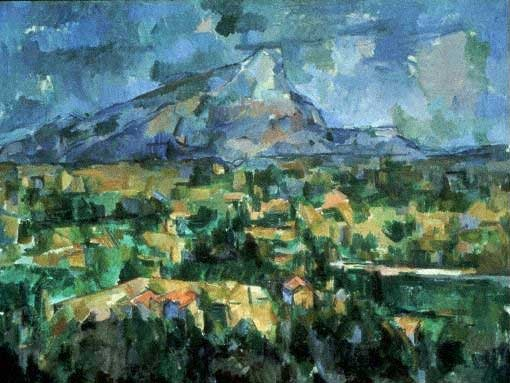
\includegraphics[width=1.0\textwidth]{images/cezanne1.jpg}
	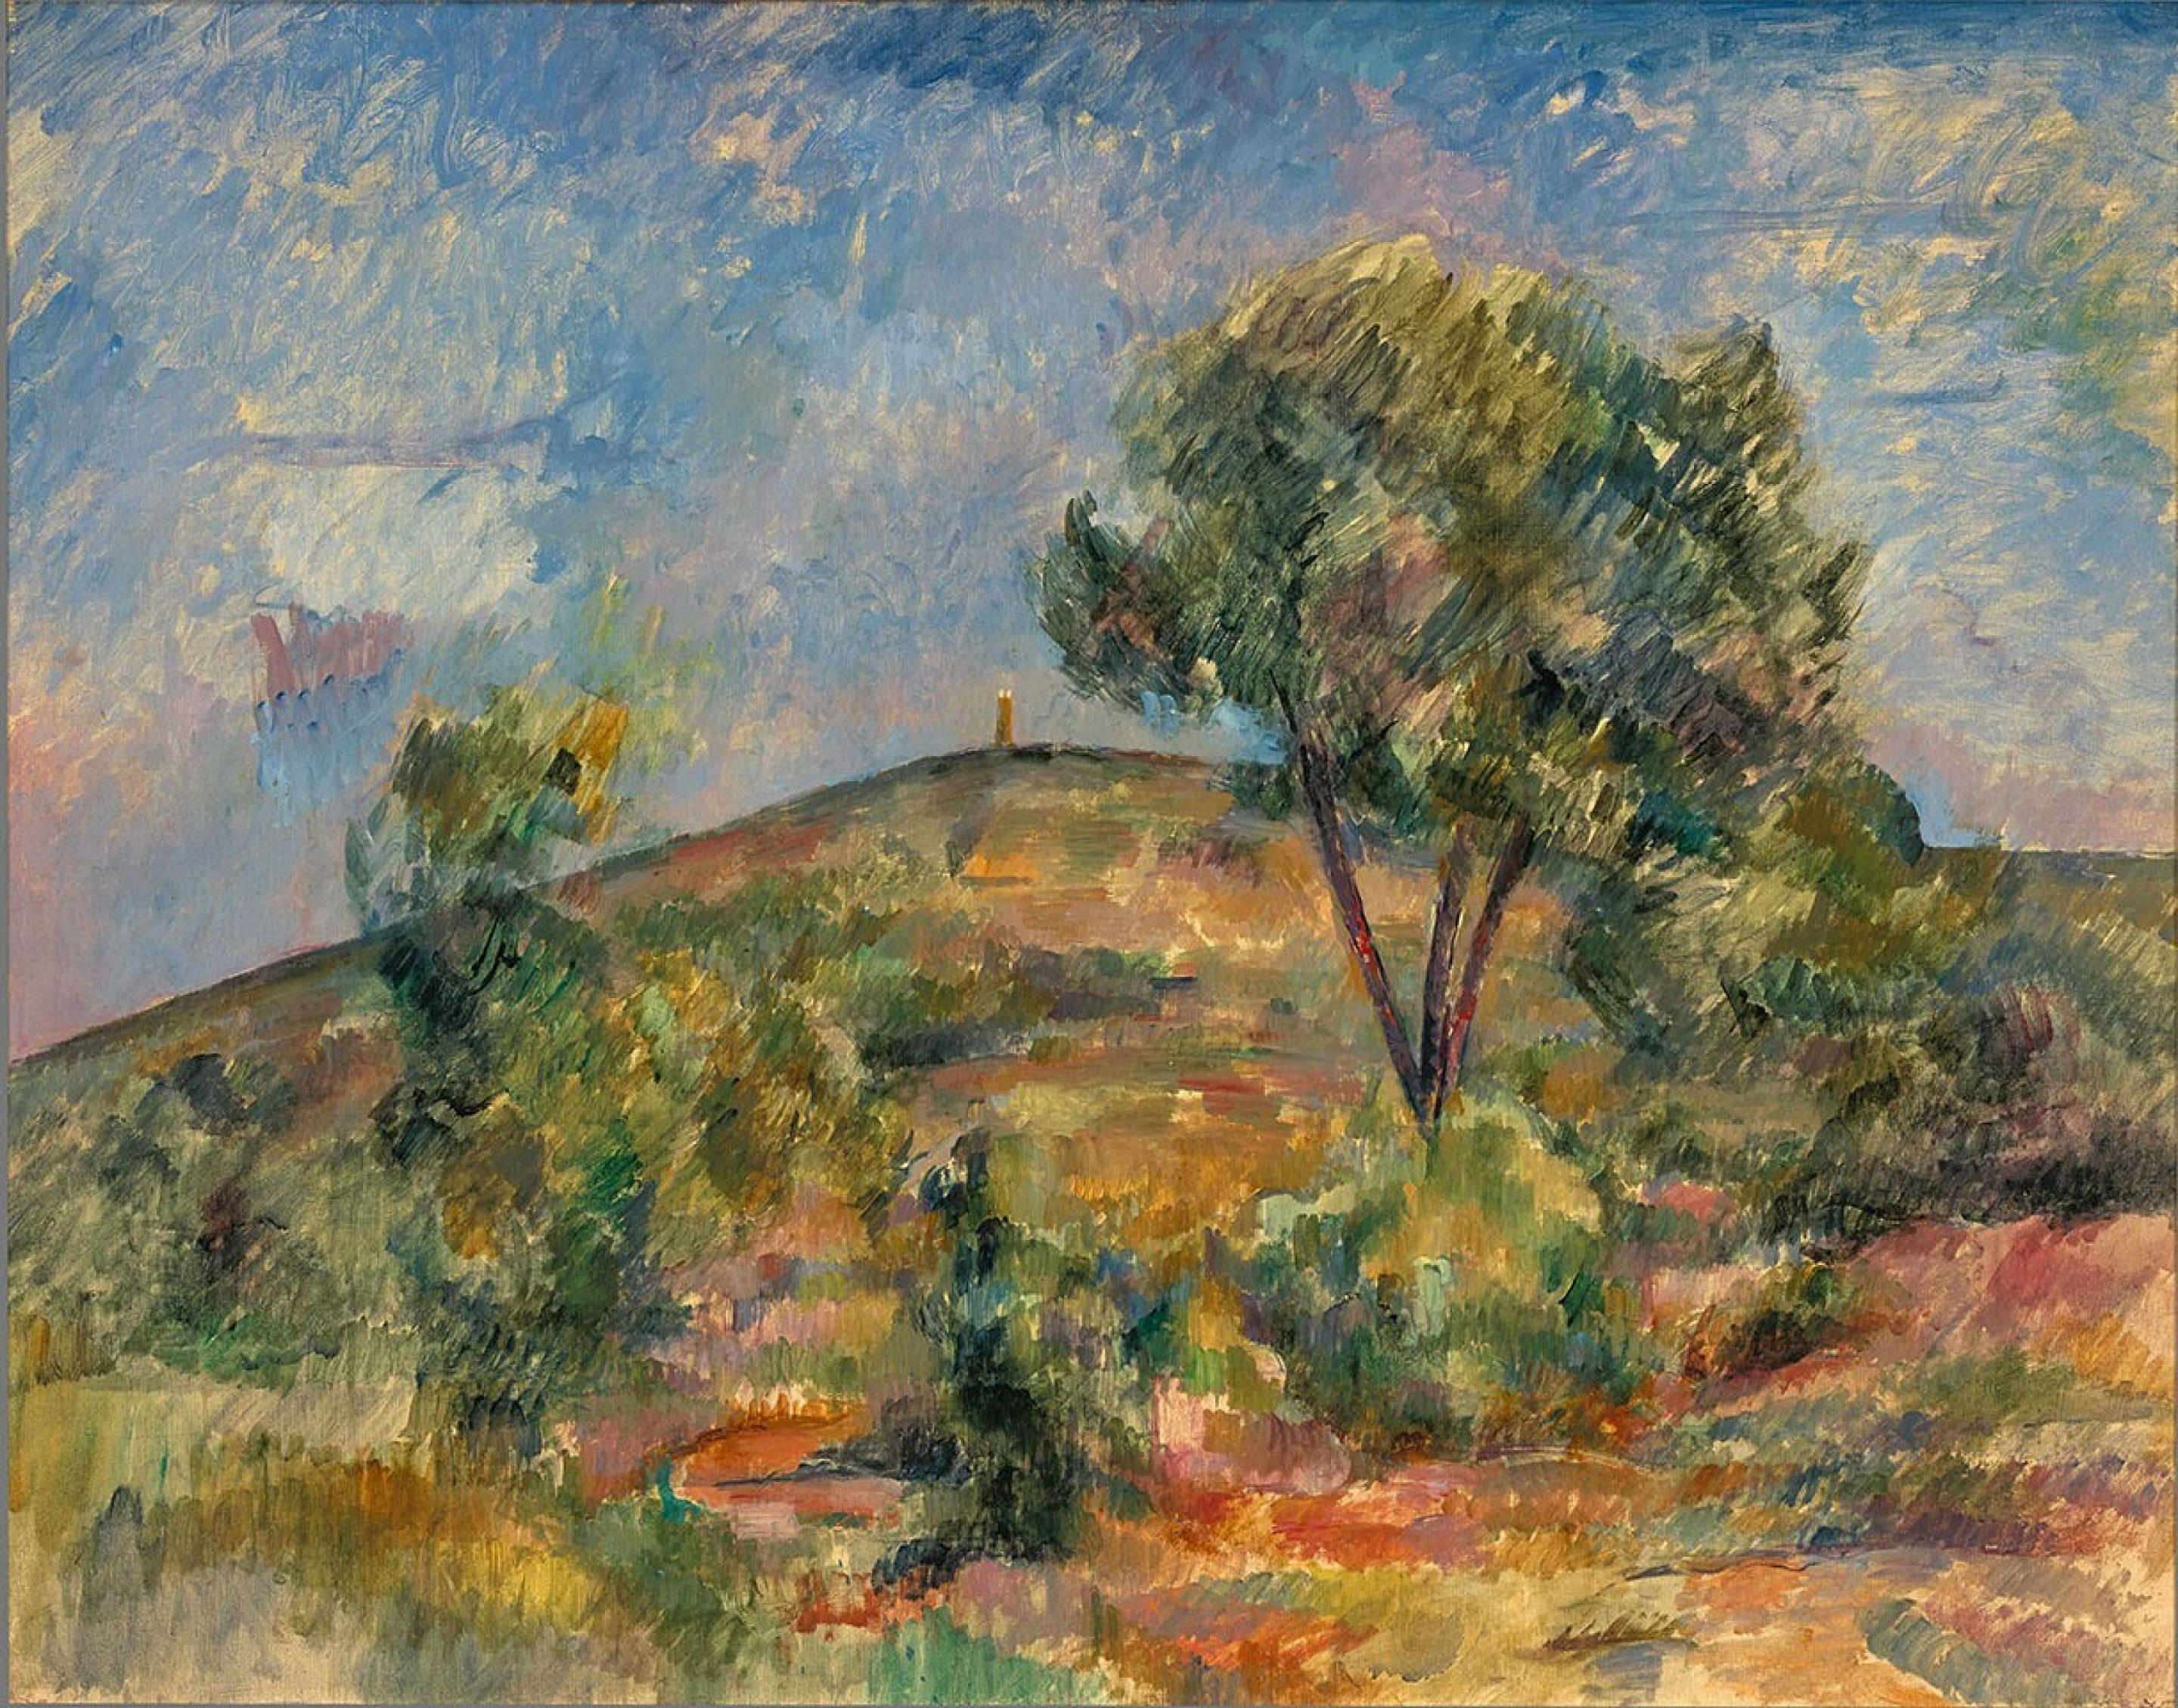
\includegraphics[width=1.0\textwidth]{images/cezanne2.jpg}
	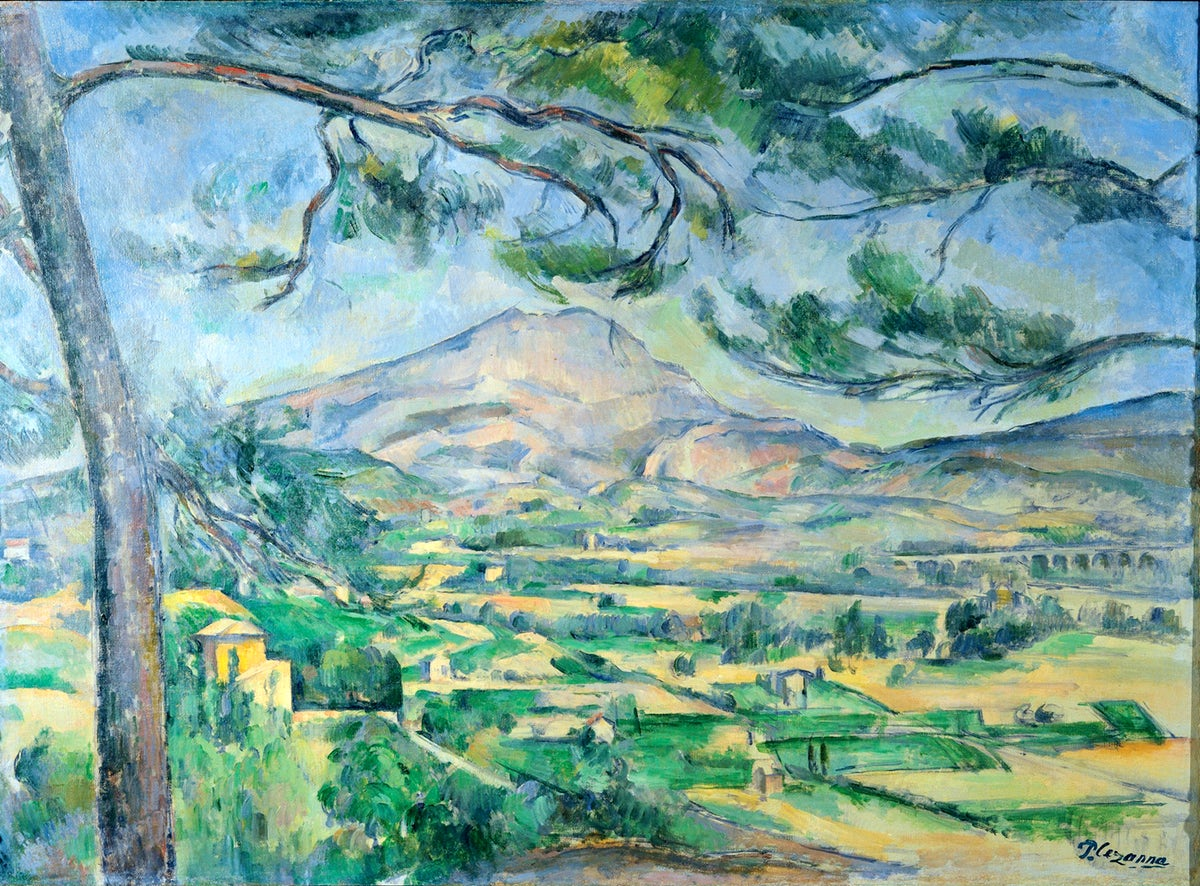
\includegraphics[width=1.0\textwidth]{images/cezanne3.jpg}
	\column{0.3\textwidth}
	\centering
	Who painted that?
	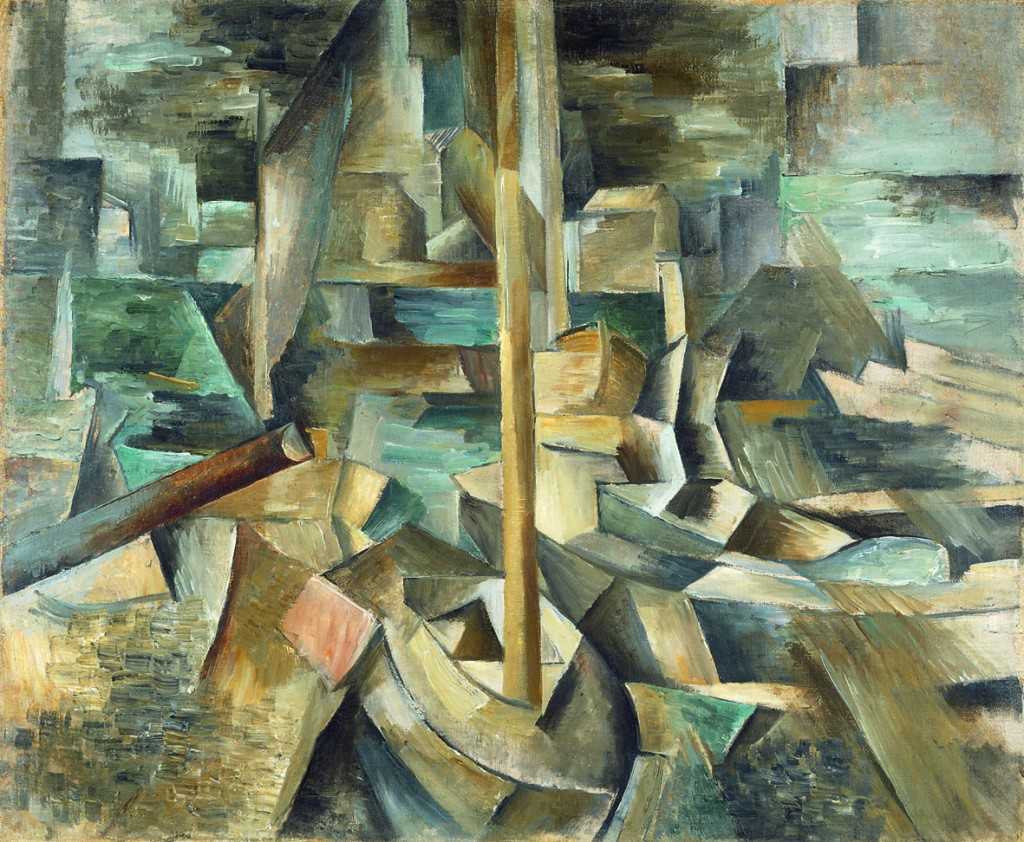
\includegraphics[width=1.0\textwidth]{images/Braque4.jpg}
	
	\pause
	Most likely most of you can identify the painter correctly, 
	although I presented only three pictures of each.
\end{columns}

\end{frame}
%-----------------------------------------------------------------------
%-----------------------------------------------------------------------
\begin{frame}[c]{Recap Supervised Learning}

Dataset:
\begin{equation}
\dataset = \{(x_1, y_1), \ldots, (x_k, y_k) \}
\end{equation}

\bigskip
\pause

Learning a model $\phi$ (e.g., weights of a neural network):
\begin{eqnarray}
\argmax_{\phi} \log p(\phi|\dataset)\\
= \argmax_{\phi} \log p(\dataset | \phi) + \log p(\phi) \\
= \argmax_{\phi} \sum_i \log p(y_i | x_i, \phi) + \log p(\phi)
\end{eqnarray}

Challenge:
\begin{itemize}
	\item Learning starts from scratch\\
	(e.g., we initially have no clue how to learn a good $\phi$)
	\item we might only have very few examples in $\dataset$ 
	(i.e., $k$ is small)
\end{itemize}

\end{frame}
%-----------------------------------------------------------------------
%-----------------------------------------------------------------------
\begin{frame}[c]{The Meta Learning Problem}

Dataset:
\begin{equation}
\dataset = \{(x_1, y_1), \ldots, (x_k, y_k) \}
\end{equation}
Set of datasets (meta-datasets):
\begin{equation}
\mdata = \{\mathcal{D}_1, \ldots, \mathcal{D}_n, \}
\end{equation}

\pause
Can we include these meta-datasets to improve learning on $\dataset$?
\begin{equation}
\argmax_{\phi} \log p(\phi|\dataset, \mdata)
\end{equation}

\pause
\medskip

\alert{Idea:} Instead of keeping $\mdata$ forever, we want to distill the knowledge into \alert{meta-parameters $\theta$}: $p(\theta|\mdata)$
 

\end{frame}
%-----------------------------------------------------------------------
%-----------------------------------------------------------------------
\begin{frame}[c]{The Meta Learning Problem}

In meta-learning, we want to learn:
\begin{eqnarray}
\argmax_{\phi} \log p(\phi|\dataset, \mdata) \\
\pause
= \argmax_{\phi} \log \int_{\Theta} p(\phi \mid \dataset, \theta) p(\theta \mid \mdata) d\theta\\
\pause
\approx \argmax_{\phi} \log p(\phi | \dataset, \theta^*) + \log p(\theta^* | \mdata)\\
\pause
= \argmax_{\phi} \log p(\phi | \dataset, \theta^*)
\end{eqnarray}

\pause

The meta-learning problem is:
\begin{equation}
\argmax_{\theta} \log p(\theta | \mdata)
\end{equation}


\end{frame}
%-----------------------------------------------------------------------
%-----------------------------------------------------------------------
\begin{frame}[c]{AutoML $\subset$ Meta Learning}

\begin{itemize}
	\item AutoML can be seen as special case of meta learning
	\pause
	\medskip
	\item $\theta$ could be:
	\begin{itemize}
		\item a hyperparameter configuration ($\lambda$) 
		\item a neural network architecture
	\end{itemize}
	\pause
	\medskip
	\item What would be $\mdata$ here?
	\begin{itemize}
		\item the train and validation dataset?
		\item a dataset on which we optimized $\lambda$ (e.g., CIFAR-10)\\ such that we can use it on another dataset (e.g., imagenet)
	\end{itemize}
\end{itemize}	

\end{frame}
%-----------------------------------------------------------------------
%-----------------------------------------------------------------------
\begin{frame}[c]{Meta Learning $\subset$ AutoML}

\begin{itemize}
	\item Meta learning can be powerful to complement AutoML
	\pause
	\medskip
	\item we can learn a a lot of things $\mdata$ to improve the performance on new datasets
	\begin{itemize}
		\item pre-initialization of networks weights\\
		(e.g., pre-train on imagenet and fine-tune on a new dataset)
		\item learning a meta-DNN to predict how to train another target-DNN\\
		(more next week)
	\end{itemize}
	\pause
	\medskip
	\item Open question: If we can learn how to learn,\\ do we need AutoML anymore?
\end{itemize}

\end{frame}
%-----------------------------------------------------------------------
%-----------------------------------------------------------------------
\section{Algorithm Selection}
%----------------------------------------------------------------------
\begin{frame}[c]{Idea: Algorithm Selection}

\begin{itemize}
	\item By applying ML to many different datasets,\\
	humans get an intuition \alert{what works well on which dataset}
	\pause
	\item E.g., humans came up with rule of thumbs:\\
	"On small datasets, we use a SVM, on mid-size dataset a RF 
	and on big data a DNN"
	\pause
	\item Although these rule thumbs are quite useful,
	they are often not correct and too strongly simplified
	\pause
	\item \alert{Question}: Can we learn from data which algorithm we should use for a given dataset?
\end{itemize}


\end{frame}
%-----------------------------------------------------------------------
%----------------------------------------------------------------------
\begin{frame}[c]{Definition: Algorithm Selection \litw{Rice 1976}}

\begin{block}{Definition}
	Given 
	\begin{itemize}
		\item a \alert{distribution} $\mdata$ of meta datasets,
		\item a portfolio of algorithms $\algo \in \portfolio$,
		\item and a cost metric $c:  \portfolio \times \mdata \rightarrow \perf$,   
	\end{itemize}
	
	the \emph{per-instance algorithm selection problem} is to find a mapping 
	$s: \dataset \mapsto \algo$ 
	that optimizes 
	$$\int_{\mdata} c(s(\dataset),\dataset) p(\dataset)  d\dataset$$
\end{block}

\bigskip
\pause


\end{frame}
%-----------------------------------------------------------------------
%----------------------------------------------------------------------
\begin{frame}[c]{Meta Features in Machine Learning}
	
To learn the mapping $s: \dataset \mapsto \algo$, we need a way to represent $\dataset$

\begin{center}
	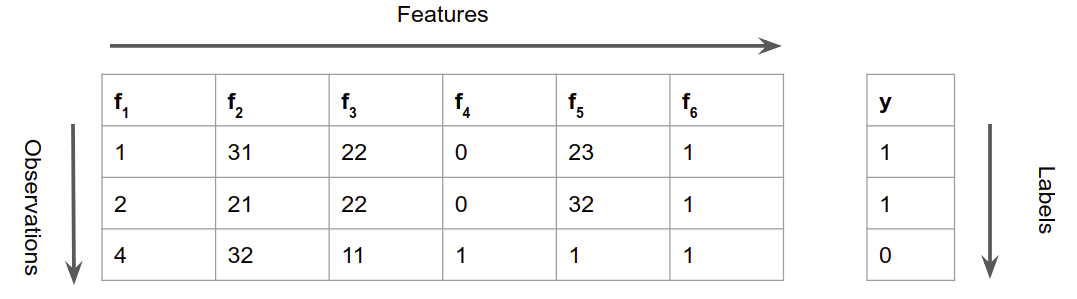
\includegraphics[width=0.7\textwidth]{images/ml_data}
\end{center}


What kind of ``Meta features'' could describe a dataset? \hands

\pause
\begin{itemize}
	\item number of observations (samples)
	\item number of features
	\item number of classes
	\item number of categorical features
	\item number of numeric features
	\item percentage of numeric features
	\item number of missing features
	%\item number of observations belonging to most frequent class
	\item Probing: accuracy of a small decision tree
\end{itemize}
	
	
\end{frame}
%-----------------------------------------------------------------------
%----------------------------------------------------------------------
\begin{frame}[c]{Meta Features in Machine Learning}

To learn the mapping $s: \dataset \mapsto \algo$, we need a way to represent $\dataset$

\begin{center}
	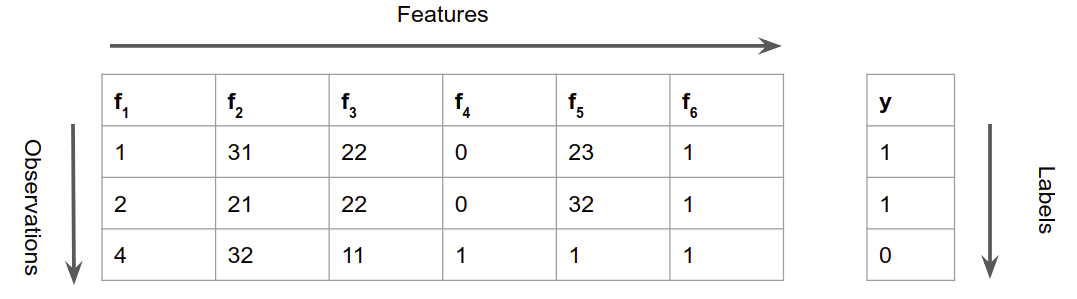
\includegraphics[width=0.7\textwidth]{images/ml_data}
\end{center}


What kind of ``Meta features'' could describe a dataset? \hands

\pause
\begin{itemize}
	\item number of observations (samples)
	\item number of features
	\item number of classes
	\item number of categorical features
	\item number of numeric features
	\item percentage of numeric features
	\item number of missing features
	%\item number of observations belonging to most frequent class
	\item Probing: accuracy of a small decision tree
\end{itemize}


\end{frame}
%-----------------------------------------------------------------------
%----------------------------------------------------------------------
\begin{frame}[c]{Assumptions for Traditional Algorithm Selection}

We assume for a discrete set of datasets from $\mdata$ that
\begin{itemize}
	\item we have pre-computed the meta features on all datasets
	\pause
	\begin{itemize}
		\item if our cost metric is not related to runtime,\\
		we assume that the cost for computing the meta features is\\ negligible compared to training a model
	\end{itemize}
	\pause
	\item we have measured the cost $c(\algo, \dataset)$ on all possible pairs $\langle \algo, \dataset\rangle$
\end{itemize}

\pause
\medskip

$\leadsto$ We have two matrices as training data,\\ one with meta-features and one with cost values

\end{frame}
%-----------------------------------------------------------------------
%----------------------------------------------------------------------
\begin{frame}[c]{Algorithm Selection as a Regression Problem}

\begin{itemize}
	\item Given a new dataset and its meta-features $f(\dataset)$
	\item we "only" need to predict the performance of all algorithms $\algo \in \portfolio$
	\item Train for each algorithm $\algo \in \portfolio$, a regression model to predict its cost $c(\dataset)$ given the meta features:
	$$\hat{m}_\algo: f(\dataset) \mapsto c(\algo, \dataset) $$
	\pause
	\item Selection for given test $\dataset_{\text{test}}$:
	$$\argmin_{\algo \in \portfolio} \hat{m}_\algo(f(\dataset_{\text{test}}))$$
	\pause
	\item Remarks:
	\begin{itemize}
		\item As regression model, we can use essential whatever you want\\
		e.g., ridge regression, a random forest or a neural network
		\item We could also train one joint model, we indicator features of the algorithms
	\end{itemize}
\end{itemize}


\end{frame}
%-----------------------------------------------------------------------
%----------------------------------------------------------------------
\begin{frame}[c]{Algorithm Selection as a Classification Problem}

\begin{itemize}
	\item Learning a regression problem is an indirect approach solving the algorithm selection problem
	\pause
	\item Can we directly solve the multi-class classification problem?
	$$s: \dataset \mapsto \algo$$
	\pause
	\item We can use common approach for multi-class classification
	\item Algorithm selection has special characteristic:\\
	\alert{Some datasets are more sensitive to algorithm selection than others}
	
\end{itemize}


\end{frame}
%-----------------------------------------------------------------------
%----------------------------------------------------------------------
\begin{frame}[c]{Pairwise Cost-Sensitive Classification Problem \litw{Xu et al. 2011}}

\begin{itemize}
	\item The sensitivity of a dataset $\dataset$ to algorithm selection across a portfolio is somehow hard to measure
	\pause
	\item For each pair of algorithms $\langle \algo_i, \algo_j \rangle$ we can easily measure the sensitivity by
	$$sim(\dataset, \algo_i, \algo_j) = || c(\algo_i, \dataset) - c(\algo_j, \dataset) ||$$
	\pause
	\item Train for each pair of algorithms a classification model $s_{ \algo_i, \algo_j}$ predicting which algorithm performs better
	\item consider for each training dataset $\dataset_{\text{train}}$ the $sim(\dataset_{\text{train}}, \algo_i, \algo_j)$
	\begin{itemize}
		\item cost-sensitive classification is often possible by modifying the loss function or split metric in tree-based approaches
	\end{itemize}
	\item Selection for given test $\dataset_{\text{test}}$:
	$$\argmax_{\algo \in \portfolio} \sum_{\algo' \in \portfolio} s_{\algo, \algo'}(f(\dataset_{\text{test}})) $$
	
\end{itemize}

\end{frame}
%-----------------------------------------------------------------------
%----------------------------------------------------------------------
\begin{frame}[c]{Remarks on Algorithm Selection}

\begin{itemize}
	\item Pairwise cost-sensitive classification requires $\sim |\portfolio|^2$ models
	\pause
	\item From our experience, pairwise cost-sensitive approaches perform often better than regression approaches, but not always
	\pause
	\item We use machine learning to optimize machine learning
	\begin{itemize}
		\item Also the meta learning level can benefit from AutoML\\ \lit{Lindauer et al. 2015}
	\end{itemize}
	\pause
	\item Algorithm selection is not limited to machine learning
	\item Algorithm selection can be applied to any algorithm class where 
	\begin{enumerate}
		\item we have a discrete portfolio of algorithms to choose from
		\item the tasks (aka. datasets) are sensitive to the algorithm choice (so called heterogeneous instances)
	\end{enumerate}
	\pause
	\item There is a benchmark library for algorithm selection data called ASlib (\url{www.aslib.net}) \lit{Bischl et al. 2016}
\end{itemize}

\end{frame}
%-----------------------------------------------------------------------
%-----------------------------------------------------------------------
\section{AutoML Warmstarting}
%----------------------------------------------------------------------
\begin{frame}[c]{Warmstarting}

\begin{itemize}
	\item Recap: Instead of starting from a random configuration we often start from a expert-defined configuration for hyperparameter optimization (HPO)
	\pause
	\item We also know that the default configuration often does not perform well on a new dataset
	\begin{itemize}
		\item Otherwise there would be no point in HPO
	\end{itemize}
	\pause
	\item Question:\\ \alert{Can we learn from previous datasets $\mdata$ how to initialize HPO?}
	\begin{itemize}
		\item the same ideas also apply to NAS
		\item for simplicity we focus on HPO 
	\end{itemize}
\end{itemize}

\end{frame}
%-----------------------------------------------------------------------
%----------------------------------------------------------------------
\begin{frame}[c]{Multi-Configuration Initialization}

\begin{itemize}
	\item Idea: Instead of a single starting point, use a \alert{portfolio $\Lambda_{init}$} as an initial design
	\item Assume that we applied HPO already to many datasets $\mdata$ and\\
	obtained a well-performing configuration on all of them $\hat{\lambda}_\dataset$
	\item Straightforward idea: 
	$$\Lambda_{init} = \bigcup_{\dataset \in \mdata} \{ \hat{\lambda}_\dataset \}$$
	\item Problems:
	\begin{itemize}
		\item If $|\mdata|$ is too large, HPO will be dominated by $\Lambda_{init}$
		\item $\Lambda_{init}$ has potentially a lot of similar configurations\\
		$\leadsto$ $\Lambda_{init}$ is not complementary
	\end{itemize}
\end{itemize}


\end{frame}
%-----------------------------------------------------------------------
%-----------------------------------------------------------------------
\section{Few Shot Learning}
%----------------------------------------------------------------------
\begin{frame}[c]{XXX}



\end{frame}
%-----------------------------------------------------------------------
%-----------------------------------------------------------------------
\section{Learning to Learn/Optimize}
%----------------------------------------------------------------------
\begin{frame}[c]{XXX}



\end{frame}
%-----------------------------------------------------------------------

%----------------------------------------------------------------------
\begin{frame}[c]{Learning Goals}

After this lecture, you are able to \ldots

\begin{itemize}
	\item ...
\end{itemize}
\end{frame}
%-----------------------------------------------------------------------

%----------------------------------------------------------------------
\begin{frame}[c]{Literature [These are links]}

\begin{itemize}
	\item \lit{\href{}{}}	
\end{itemize}

\end{frame}
%----------------------------------------------------------------------


